\chapter{Evaluation}
kapitelstarttext...
\section{Simulationsaufbau}
Zunächst wird auf den Aufbau des verwendeten Simulators eingegangen, sowie auf die ,in der Simulationen verwendeten, Daten.
\subsection{Simulationsframework und Simulatoren}
Für die Durchführung der Simulation der in Kapitel 3 vorgestellten Methodiken wird die co-Simulations Software Mosaik \footnote{https://mosaik.offis.de/} verwendet. Der Mosiak Simulator wurde speziell für Simulation von Smart Grid-Anwendung entwickelt und eignet sich deswegen hervorragend für die im Zuge dieser Arbeit zu erfüllenden Aufgaben. Der Simulator unterstütz zudem die schchnelle Einbing von einem Framework namens PYPOWER. PYPOWER wurde zur Simulation von Stromflüssen entwickelt und ist in der Lage anhand eines Stromnetzes die Ströme der elektrischen Energie zu simulieren. Diese Simulationdes Stromflusses schließt auch den Transportverlust der Niederspannung und den Zusammenhang von Wirk- zu Blindleistung mit ein. Die Art der Integration von PYPOWER in die Mosaik co-Simulations Software, sorgt dafür, dass ein Nutzer PYPOWER nicht außergewöhnlich konfigurieren muss. Ein Stromnetz welches an Mosaik übergeben wird, wird automatisch PYPOWER mitverwenden. Das Stromnetz welches in dieser Arbeit verwendet wird ist ein standardisiertes europäisches Niederspannungsnetz, welches von der IEEE, dem Institut für Elektro- und Elektronikingenieure, für solche Simulation herausgegeben wurde, um Ergebnisse auf einer EU-weiten Ebene vergleichbarer zu machen. Die Methodiken um den Stromfluss im Niederspannungsnetz zu beeinflussen wurden im Kapitel 3 vorgestellt. Dieser Teil des Simulators ist auch der einzige Teil welcher zwischen den verschiedenen Simulationen ausgetauscht wird. Der letzte Baustein welcher für die Simulation benötigt wird, sind die Fahrzeuge, welche geladen werden sollen. Dieser Simulator ist in der Lage anhand der aus dem Netz abgerufen Leistung und der Zeit zu bestimmen, wie sich die Fahrzeugparameter verändern. Die verschiedenen Teile des Simulators benötigen an manchen Stellen Daten von anderen Teilen des Simulators. Die Methodiken, welche in dieser Arbeit entwickelt wurden setzen an den Anschlusspunkten des Niederspannungsnetzes für Privatverbraucher an. Über diese Anschlusspunkte wird unter anderem die Leistung bezogen, welche für das laden der mit diesem Anschlusspunkt verbunden Elektrofahrzeuge verwendet wird. Die aktuell verwendete Methodik erhält vom jeweiligen Anschlusspunkt die aktuell anliegende Spannung. Die mit dem jeweiligen Anschlusspunkt verbunden Elektrofahrzeuge, teilen der Methodik die Ankunftszeit, den Abfahrtszeitunkt, die aktuell möglich Stromstärke beim Laden, sowie den aktuellen Ladestand mit. Das jeweilige Elektrofahrzeug bezieht dann die von der Methodik berechnete mögliche Ladeleistung aus dem Netz, teilt diesem also die Höhe der bezogenen Leistung mit. Die Transformatorlast wird über ein Broadcastsystem vom Transformator aus verteilt, Die Teilnehmeranzahl kann von jeder Methodik, anhand der erhaltenen Nachrichten bestimmt werden. Diese Nachrichten wurden wiederrum von anderen Teilnehmer versandt.\\
\begin{figure}[htb]
\centering
	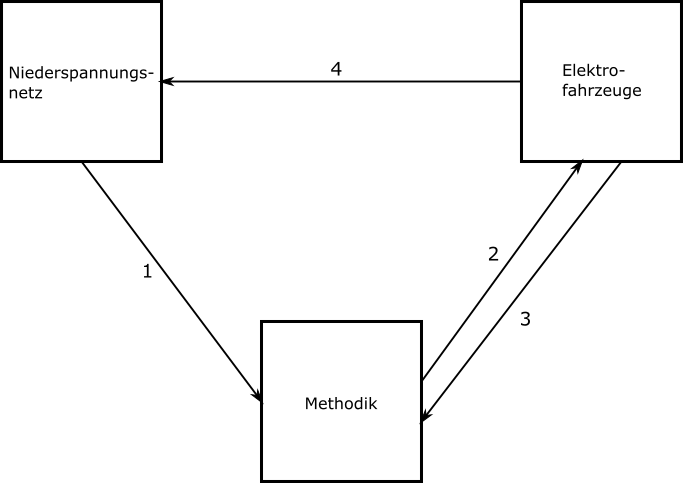
\includegraphics[width=0.5\textwidth]{img/SimAufbau1.png}
	\caption{Schnittstellen zwischen den Teilen des Simulators}
	\label{Abb_SimAufbau}
\end{figure}

In der Abbildung \ref{Abb_SimAufbau} wird ersichtlich wer welche Daten an wen weitergibt. Die mit der eins markierte Verbindung stellt die Weitergabe von Daten  vom Niederspannungsnetz an die aktuelle verwendete Methodik dar. Dabei wird die aktuell am Anschlusspunkt gemessene Spannung weitergegeben. Die zwei mit zwei und drei markierten Übergänge verdeutlichen den Datenaustausch zwischen der verwendeten Methodik und dem angeschlossen Elektrofahrzeug. Das Elektrofahrzeug sendet die Ankunftszeit, die Abfahrtszeit, die aktuell maximal mögliche Stromstärke und den Ladezustand an die Methodik und erhält im Gegenzug die aktuelle Höhe der aus dem Netz beziehbaren Leistung. Über die Verbindung, welche mit 4 markiert ist, wird dem Netz von Elektrofahrzeug mitgeteilt, welche Leistung aktuell aus dem Netz bezogen wird.
\subsection{Annahmen und verwendete Daten}
Im Zuge dieser Arbeit wird eine nicht unerhebliche Menge an Daten verarbeitet. Die Mehrheit dieser Daten steht in Zusammenhang mit den Elektrofahrzeugen. Die Daten die diese für die Simulation zur Verfügung stellen, wurden vom Deutschem Zentrum für Luft – und Raumfahrt erhoben. Diese Erhebung fand im Zuge einer Mobilitätsstudie statt. Es wurden Teilnehmer für diese Studie aus der Bevölkerung ausgewählt, welche dann ihr Mobilitätsverhalten dokumentiert haben. Diese Mobilitätsverhalten dienen als Grundlage für die Daten der verwendeten Elektrofahrzeuge. Durch die Auswertung dieser Daten wurden Ankunfts- und Abfahrtszeiten, sowie die jeweils gefahrene Wegstrecke bestimmt. Durch die Länge der Wegstrecke kann bestimmt werden wie viel des Ladezustandes auf dieser Strecke verbraucht wird und somit auch der Ladestand bei Ankunft an der Ladestation.\\
Es werden für die Simulationen auch einige Annahmen getroffen. Der Kapazität der Batterie, in welcher die elektrische Energie der Elektrofahrzeuge gespeichert wird, wird auf 36253,11 Wh festgelegt. Dieser Wert durch Auswertung zweier Statistiken ermittelt, welche die meistzugelassen Elektrofahrzeuge in Deutschland beinhalteten und die Batteriekapazität pro Modell. Durch die Verwendung dieser Statistiken wurde eine durchschnittliche Batteriekapazität der Elektrofahrzeuge in Deutschland ermittelt. Dieser Mittelwert stellt einen Kompromiss zu einer individuellen Batteriekapazität dar, stellt allerdings auch sicher vergleichbare Ergebnisse zu erhalten. Die Norm DIN EN 50150 setzt die Normspannung im Deutschem Stromnetz auf 230 Volt, daher wird dieser auch in dieser Arbeit verwendet. Die maximale Trafolast wurde durch eine Simulation ohne Aktivität von Elektrofahrzeugen ermittelt. Die, in dieser Simulation gemessene, Transformatorlast wurde verdoppelt. Diese Verdopplung soll die Belastung des Transformators so gering wie möglich halten, den Ladevorgängen aber dennoch die Möglichkeit bieten auch Leistung abzurufen. Eine weitere Annahme ist die maximale Anzahl an Elektrofahrzeugen, hierbei wurde davon ausgegangen, das ein jeder Haushalt im Niederspannungsnetz über exakt zwei Elektrofahrzeuge verfügt, welche mithilfe eine 22kW Ladegeräts geladen werden. Diese Annahme geht aus Statistiken eines Bundesamtes zurück, welche aussagt, das in ländlich geprägten Gebieten vermehrt größere Haushaltemit zwei oder mehr Personen auftreten. Aus Gründer der Normalisierung zwischen den Anschlusspunkten ans Niederspannungsnetz, wird daher immer von zwei Fahrzeugen je Anschlusspunkt ausgegangen. bei dem in dieser Arbeit verwendtem Netz dem IEEE906 gibt es 55 Anschlüsse für Haushalte, folglich wird von 110 Elektrofahrzeugen ausgegangen.

\section{Simulationsergebnisse}
Die Ergebnisse der Simulationen werden zunächst aufgeteilt auf die verwendeten Methodiken vorgestellt. Eingegangen wird auf die verursachte Trafolast, die Spannungen, aufgetretene und behandelte Kollisionen, sowie die Qualitätserfahrungen und die Fairness zwischen den Ladevorgängen. 
\subsection{VDE alleine}
Die Verwendung des VDE-Spannungscontrollers (\ref{capBody:VDE}) wurde über einen Zeitraum von einer Woche hinweg simuliert, dargestellt werden die Ergebnisse eines einzelnen Werktages. Ein Werktag wurde gewählt, da die Mehrheit der simulierten Tage ein Werktag ist. Dargestellt wird die Transformatorlast, die minimalen Werte der Spannung sowie die Anzahl der Teilnehmer, welche Leistung aus dem Netz beziehen. 
\begin{figure}[htb]
\centering
	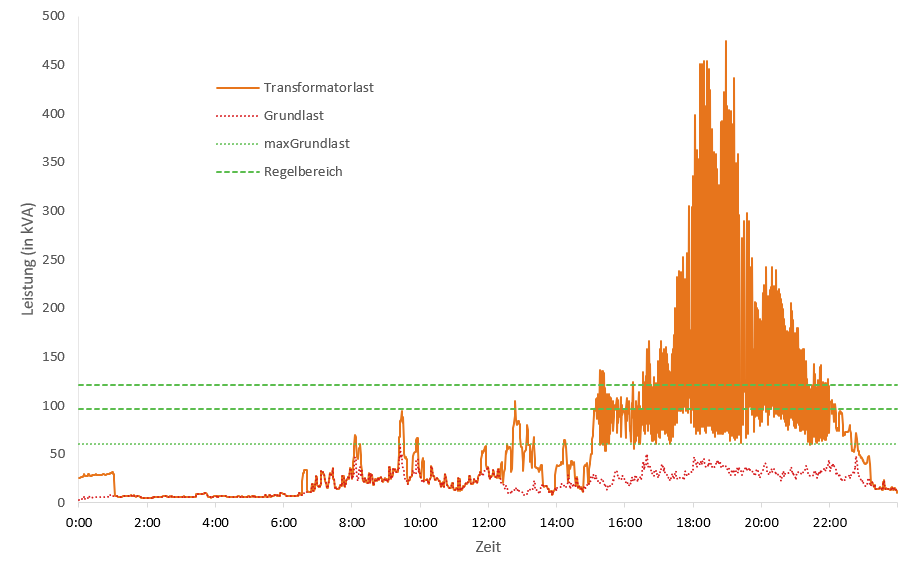
\includegraphics[scale=0.7]{img/VDE_tau/TrafoLast7.png}
	\caption{Trafolast bei Verwendung des VDE Spannungs-Controllers}
	\label{Abb_VDEtauTrafoLast}
\end{figure}

In der Abbildung \ref{Abb_VDEtauTrafoLast} ist die vom Transformator ans Niederspannungsnetz abgegeben Scheinleistung in kVA über den Verlauf eines Tages abgebildet. Der Regelbereich des Controllers ist im Falle der Transformatorlast nicht relevant, der VDE Controller lediglich die Spannung berücksichtigt.
\begin{figure}[htb]
\centering
	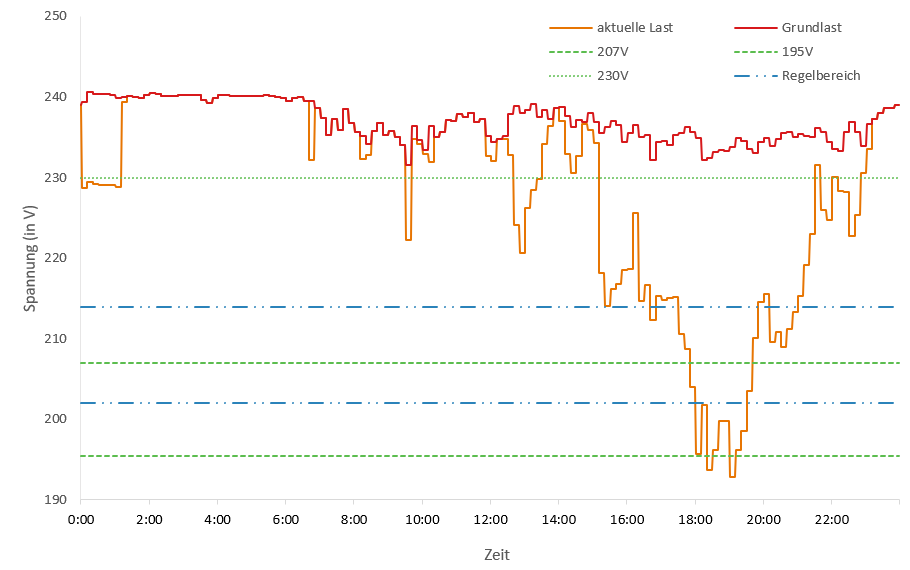
\includegraphics[scale=0.7]{img/VDE_tau/Spannung10m6.png}
	\caption{Spannungsverlauf mit 10 Minuten Mittelwerten bei Verwendung des VDE Spannungs-Controllers}
	\label{Abb_VDEtauSpannung10m}
\end{figure}

In der Abbildung \ref{Abb_VDEtauSpannung10m} ist der Verlauf der minimalen Spannung über das gesamte Niederspannungsnetz hinweg aufgezeichnet. Bei den dargestellten Werten handelt es sich nicht um minutengenaue Messwerte, sondern um die Mittelwerte von 10 Minuten Intervallen. Diese Intervalle wurden gewählt um die Erfüllung der Norm DIN EN 50160 zu bestimmen. Die Norm befasst sich allerdings mit der Spannung an einzelnen Anschlusspunkten, dargestellt werden allerdings Werte aus dem gesamten Niederspannungsnetz, somit lässt sich anhand des Graphen nur bestimmen, ob die Norm von allen Anschlusspunkten eingehalten wurde. Bei einem sichtbaren Verstoß gegen die Norm, lässt sich nur das Vorhandensein eines einzelnen Verstoßes ableiten, da nur minimal Werte dargestellt werden. Ob zeitgleich noch andere Anschlusspunkte gegen die Norm verstoßen haben ist anhand des Graphens nicht feststellbar.
\begin{figure}[htb]
\centering
	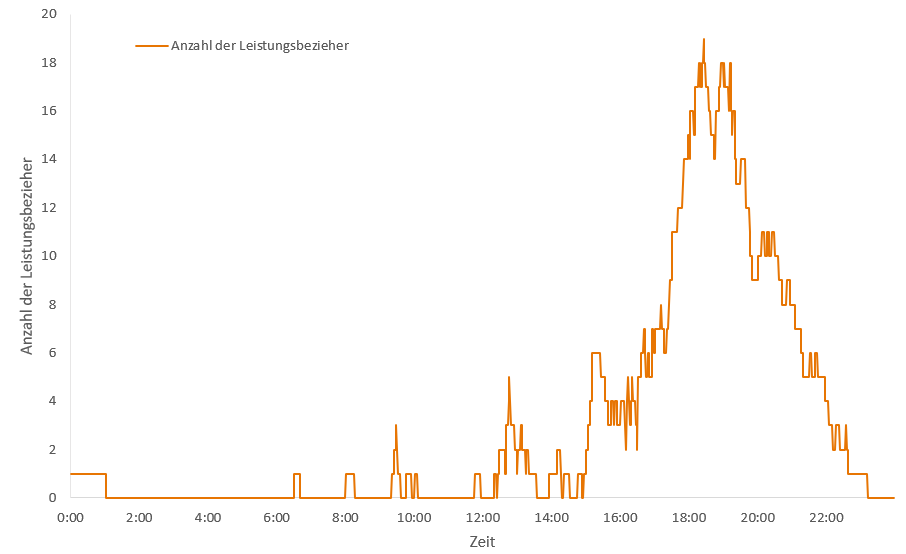
\includegraphics[scale=0.7]{img/VDE_tau/Teilnehmer.png}
	\caption{Teilnehmeranzahl bei Verwendung des VDE Spannungs-Controllers}
	\label{Abb_VDEtauTeilnehmer}
\end{figure}

In der Abbildung \ref{Abb_VDEtauTeilnehmer} ist die Anzahl an Controllern abgebildet, welche Leistung für das Laden von Elektrofahrzeugen aus dem Netz beziehen. Leistungsbezieher, welche zwar Leistung beziehen, mit dieser aber kein Elektrofahrzeug laden, werden nicht dargestellt. 
Bis etwa 16:00 steigt die bezogene Leistung am Transformator mehrmals über die Grundlast hinaus an, diese Anstiege decken sich mit einer Zunahme an Teilnehmer und sich auch an der fallenden Spannungskurve erkennbar. Die Belastungen bis zu diesem Zeitpunkt sind allerdings nicht hoch genug, dass die Spannung den Regelbereich des Spannungscontrollers erreicht. Um etwa 16:00 fällt die Spannung bis zum Beginn des Regelbereiches ab, steigt dann aber wieder an, was sich auf eine sinkende Teilnehmeranzahl zurückführen lässt. Nach 16:00 steigt die Anzahl der Teilnehmer innerhalb zweier Stunden stark an, von etwa 4 auf bis zu 18 Teilnehmer. Dieser Anstieg an Teilnehmern führt auch zu einer gesteigerten Menge an bezogener Ladeleistung. In derselben Zeit fällt auch die Spannung ab, zunächst nur bis in den Regelbereich hinein. Ab etwa 18:00 liegt die minimal gemessene Spannung unterhalb des Regelbereiches des Spannungscontrollers, etwa zwei Stunden lang werden Spannungen unterhalb des Regelbereiches gemessen. Erst als die Teilnehmerzahl ab 20:00 sinkt und damit auch die Transformatorlast wieder zurückgeht, steigt die Spannung wieder an. Der Abfall der Spannung unterhalb des Regelbereiches zeigt an, das der Spannungscontroller nicht mehr ordentlich arbeiten und nicht in der Lage ist die Spannung auf einem ausreichenden Niveau zu halten. Der Wert der Spannung der 10 Minuten Intervalle fällt auf bis zu 184,60 V ab, da dies weniger als 15 \% der Normspannung entspricht, wird die Norm DIN EN 50160 nicht erfüllt. An der Kurve der Transformatorlast lässt sich erkennen, dass der Spannungscontroller zwar arbeitet, die vorgenommen Regelungen allerdings in einer stark schwankenden Transformatorlast resultieren. \\

Die hier vorgestellte Methodik reagiert auf keine Art von Kollision, dennoch wurde die Anzahl von Situationen erfasst, in denen Kollisionen aufgetreten wären. Hierbei gibt es zu beachten, dass der Simulationszeitraum 10080 Schritte umfasst, welche von jedem der 110 betrachteten Fahrzeuge durchlaufen werden. Dies bedeutet es werden 1108800 Situationen betrachtet. In 0,13 \% davon ist eine Spannungskollision aufgetreten und in 0,15 \% davon ist eine Transformatorkollision aufgetreten. In insgesamt 0,15 \% der Fälle, also 5615 Situationen, trat eine Art von Kollisionen auf. Diese Arten der Kollisionen beinhalten eine reine Spannungskollision, eine reine Transformatorkollision, sowie eine Spannungskollision und Transformatorkollision, welche zeitgleich auftreten. \\

Innerhalb des Simulation Zeitraumes werden insgesamt 557 Ladeservices gestartet, von denen alle erfolgreich abgeschlossen wurden. Dies bedeutet, dass ein jedes Fahrzeug beim Verlassen der Ladestation einen Ladezustand von 100 \% aufwies. Beim Start eines Ladeservices lag der durchschnittliche Ladestand bei etwa 85 \%, schon nach etwa 40 \% des Ladeservices liegt der durchschnittliche Ladestand bei fast 100 \% mit einer Standardabweichung von lediglich 0,8 \%. Der schnelle Anstieg des durchschnittlichen Ladestandes zeigt das die Fahrzeuge sehr früh und gleichmäßig mit hohen Mengen an Energie versorgt werden. \\
\begin{figure}
	\begin{subfigure}{0.49\linewidth}
		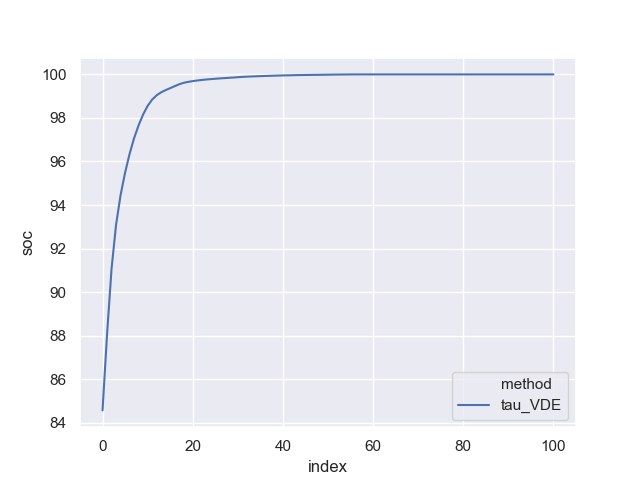
\includegraphics[width=\linewidth]{img/VDE_tau/tau_VDE_2_soc_mean.png}
        \subcaption{Durchschnittlicher Ladezustand eines Elektrofahrzeuges}
        \label{ABB_VDEtauSocMEAN}
	\end{subfigure}
	\begin{subfigure}{0.49\linewidth}
		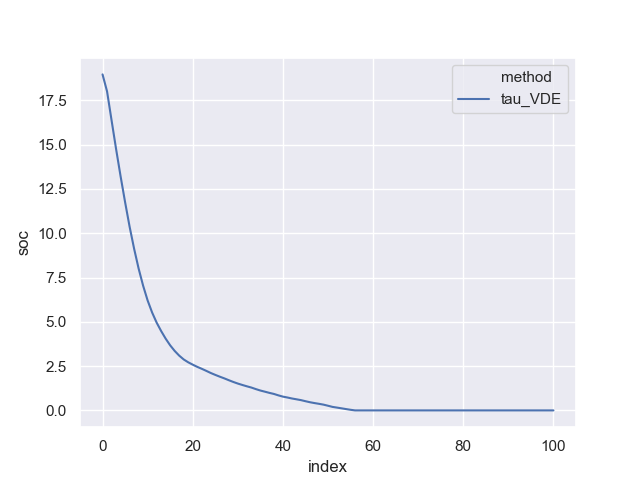
\includegraphics[width=\linewidth]{img/VDE_tau/tau_VDE_2_soc_std.png}
        \subcaption{Durschschnittliche Standardabweichung des Ladezustandes}
        \label{ABB_VDEtauSocSTD}
	\end{subfigure}
	\caption{ganz unten}
\end{figure}

Da alle begonnen Ladeservices erfolgreich beendet wurden, ist die Qualität der Ladeservices maximal. Die Fairness beim Erreichen dieser Qualität ist in Abbildung \ref{Abb_VDEtauFairness} aufgezeichnet. \\
\begin{figure}[htb]
\centering
	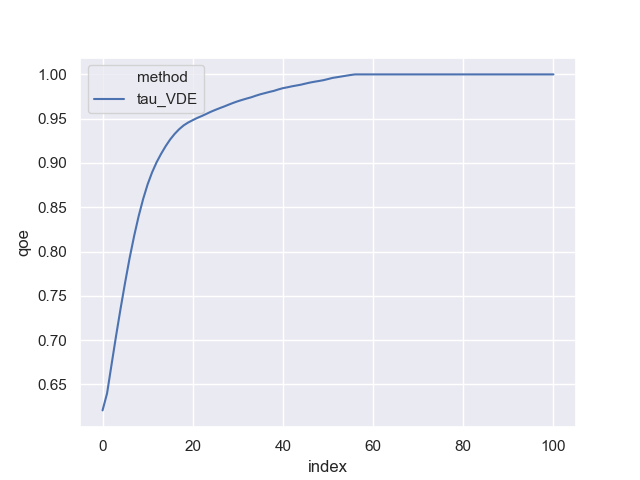
\includegraphics[scale=0.4]{img/VDE_tau/tau_VDE_2_qoe.png}
	\caption{Durchschnittlicher Qualitätserfahrung eines Elektrofahrzeuges}
	\label{Abb_VDEtauFairness}
\end{figure}

Da die Fairness abhängig von der Standardabweichung des Ladezustandes ist, steigt die Fairness wie die Standardabweichung fällt. Da, je geringer die Standardabweichung ist, desto höher ist die Fairness. Die Fahrzeuge werden bereits in den Anfangszeiten der Ladeservices mit der nötigen Energie versorgt um einen Ladestand von 100 \% zu erreichen. Da diese Erhöhung des Ladestandes bei allen Teilnehmern so schnell von statten geht, sinkt auch die Standardabweichung schnell ab. Dieses Absinken zeigt die zunehmende Ähnlichkeit der ladezustande und so auch die Fairness beim Laden.

\subsection{Slotted Aloha mit Teilnehmerzahl}
Die Verwendung von SA participants wurde über den Zeitraum von einer Woche simuliert. Da bei der Verwendung dieses Controller Wartezeiten mithilfe von Zufallszahlen bestimmt werden, wurde die Simulation mit 10 verschiedenen Startwerten für die Bestimmung dieser Zufallszahlen durchgeführt. Dargestellt werde die Ergebnisse eines einzelnen Werktages, allerdings nicht die Ergebnisse eines einzelnen Durchlaufes, sondern der Mittelwert aller Durchläufe samt der zugehörigen Standartabweichung. Es wird der selbe Werktag wie bereits in Kapitel .. verwendet, um die Vergleichbarkeit der Ergebnisse zu gewährleisten. Dargestellt wird die Transformatorlast, die minimalen Werte der Spannung sowie die Anzahl der Teilnehmer, welche Leistung aus dem Netz beziehen. \\
\begin{figure}[htb]
\centering
	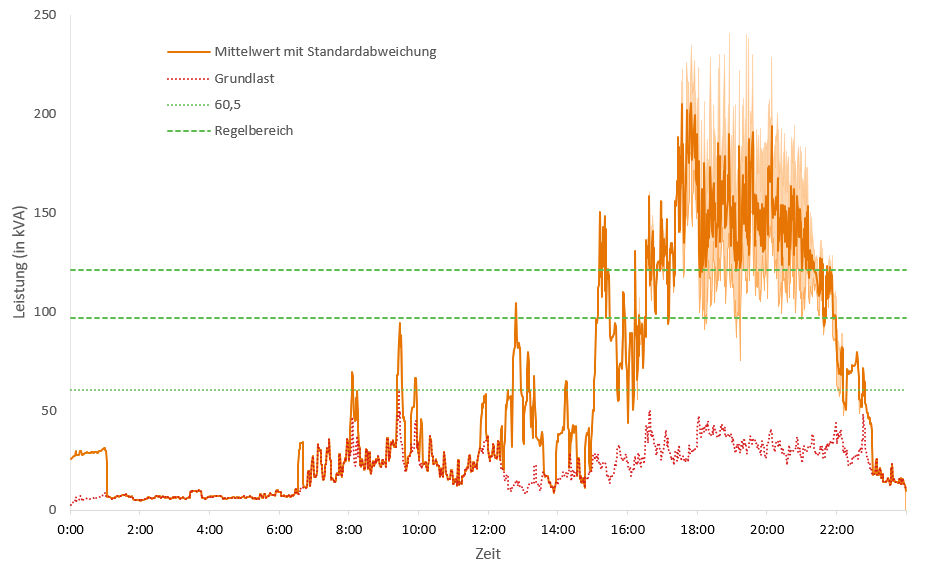
\includegraphics[scale=0.7]{img/SA_par/TrafoLast_1911_5.png}
	\caption{Trafolast bei Verwendung des Spannungs-Controllers ...}
	\label{Abb_SAparTrafoLast}
\end{figure}

In der Abbildung \ref{Abb_SAparTrafoLast} ist die vom Transformator ans Niederspannungsnetz abgegeben Scheinleistung in kVA über den Verlauf eines Tages abgebildet. Der Regelbereich des Controllers ist im Falle der Transformatorlast nicht relevant, der VDE Controller lediglich die Spannung berücksichtigt.
\begin{figure}[htb]
\centering
	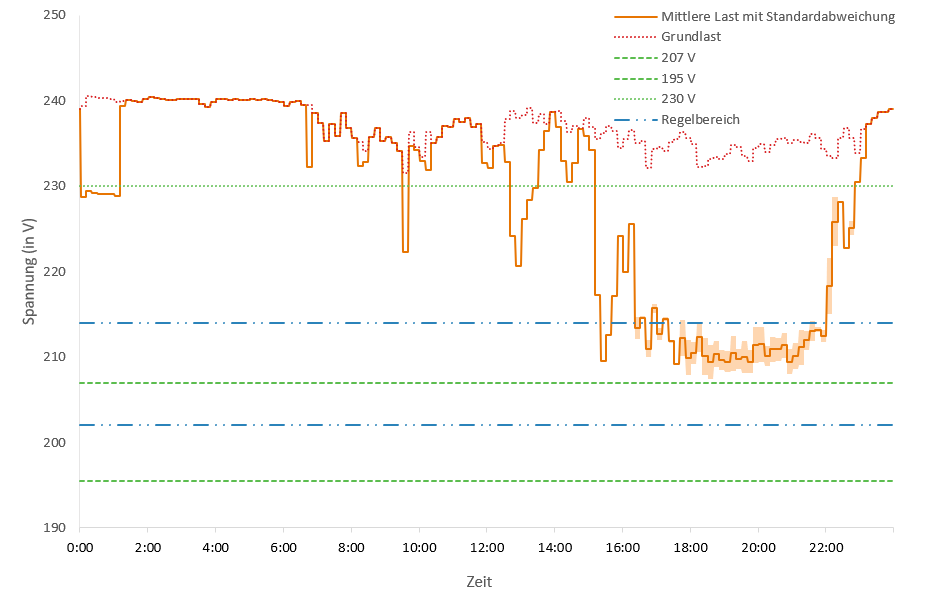
\includegraphics[scale=0.7]{img/SA_par/Vm10m7.png}
	\caption{Spannung bei Verwendung des Spannungs-Controllers ...}
	\label{Abb_SAparSpannung}
\end{figure}
Abbildung \ref{Abb_SAparSpannung} zeigt den Verlauf der minimalen Spannung über das gesamte Niederspannungsnetz hinweg. Auch hier werden die Mittelwerte von 10 Minuten Intervallen zur Überprüfung der Norm DIN EN 50160 abgebildet.
\begin{figure}[htb]
\centering
	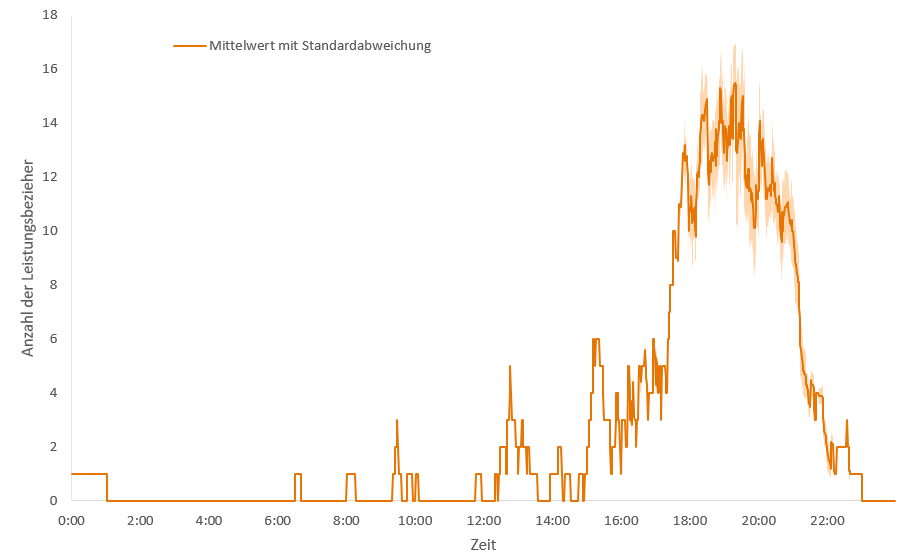
\includegraphics[scale=0.7]{img/SA_par/Teilnehmer.png}
	\caption{Teilnehmerzahl bei Verwendung des Spannungs-Controllers ...}
	\label{Abb_SAparTeilnehmer}
\end{figure}
In der Abbildung \ref{Abb_SAparTeilnehmer} ist die Anzahl an Controllern abgebildet, welche Leistung für das Laden von Elektrofahrzeugen aus dem Netz beziehen. Leistungsbezieher, welche zwar Leistung beziehen, mit dieser aber kein Elektrofahrzeug laden, werden nicht dargestellt. \\
Bis etwa 16:00 steigt sowohl die Grundlast und somit auch die Transformatorlast als ganzes zwar mehrmals an, jedoch fällt die Spannung dadurch nie bis zum Regelbereich hin ab. Um etwa 16:00 fällt die Spannung erstmals in den Regelbereich ab, steigt dann allerdings wieder an. Dieser Spannungsfall lässt sich auf einen erhöhten Leistungsbedarf von der steigenden Anzahl an Teilnehmern zurückführen. Da die Anzahl an Teilnehmer nur kurz ansteigt, steigt auch die Spannung wieder an. Nach 16:00 fällt der Minimalwert der Spannung für etwa 6 Stunden bis in den Regelbereich ab. Im selben Zeitraum kommt es auch zu einem erhöhten Leistungsabgabe am Transformator, und auch die Anzahl der Teilnehmer steigt an auf bis zu 18 Teilnehmer. Innerhalb der Zeitspanne in der sich die Spannungswerte im Regelbereich des Spannungscontrollers befinden schwanken die minimalen Werte nur gering, sie bewegen sich von 215 V bis 209 V, also innerhalb einer Spanne von 6 Volt. Diese geringe Schwankung lässt den Schluss zu das diese Variante des Controllers in der Lage ist die Spannung im Niederspannungsnetz effektiv zu regeln und auf einem ausreichenden Niveau zu halten. \\
Im gesamten betrachteten Zeitraum von einer Woche kommt es zu keiner Unterschreitung der 195 Voltmarke sowie zu lediglich im Durchschnitt etwa 0,4 Unterschreitungen der 207 Volt Marke. Die Norm DIN EN 50160 wird folglich erfüllt, da die betrachteten Grenzwerte innerhalb der erlaubten Bereiche liegen.\\
Über den Simulationszeitraum hinweg wurden im Schnitt 668,7 Situationen (+- 6,7\%) festgestellt, in denen Spannungswerte gemessen wurden, welche eine Spannungskollision verursachen könnten. In 553,9 dieser 668,7 Situationen (+- 5,9\%) trat tatsächlich eine Spannungskollision auf und eine Wartezeit wurde berechnet. Der Simulationszeitraum umfasst 10080 Zeitschritte für 110 Teilnehmer, folglich wurden 1108800 Situationen betrachtet. Die 553,9 Situationen stellen also 0,04\% der insgesamt betrachteten Situationen dar. Die hier verwendete Methodik reagiert nur auf Spannungskollisionen, die Menge von Situationen in denen eine Transformatorkollision auftreten könnte wurde dennoch erfasst. In durchschnittlich 7514,5 (+- 2,0\%) der betrachteten Situationen wurde ein Verstoß gegen den Grenzwert der Transformatorlast festgestellt, was etwa 0,67\% aller Situation entspricht.\\
\begin{figure}
	\begin{subfigure}{0.49\linewidth}
		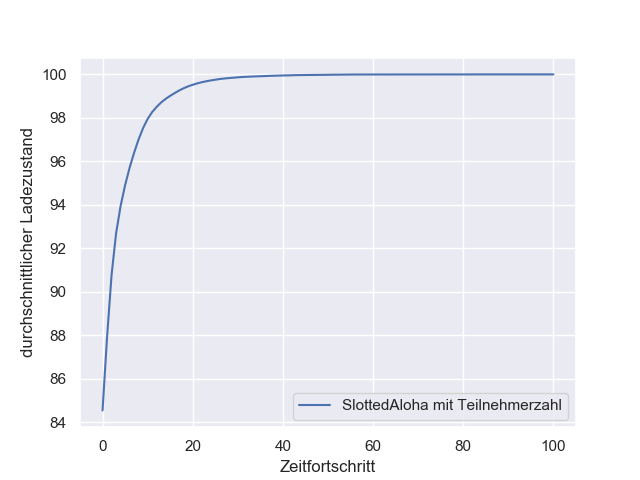
\includegraphics[width=\linewidth]{img/SA_par/SlottedAloha_participants_VDE_tau_10_soc_mean.png}
        \subcaption{Durchschnittlicher Ladezustand eines Elektrofahrzeuges}
        \label{ABB_SAparSocMEAN}
	\end{subfigure}
	\begin{subfigure}{0.49\linewidth}
		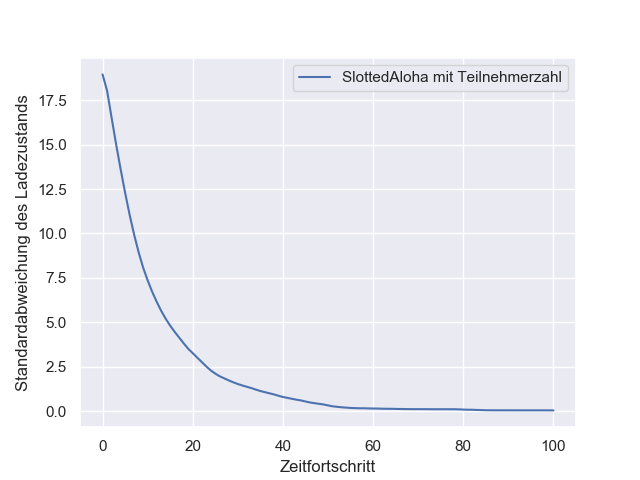
\includegraphics[width=\linewidth]{img/SA_par/SlottedAloha_participants_VDE_tau_10_soc_std.png}
        \subcaption{Durschschnittliche Standardabweichung des Ladezustandes}
        \label{ABB_SAparSocSTD}
	\end{subfigure}
	\caption{ganz unten}
\end{figure}
Alle 557 gestarteten Ladeservices wurden erfolgreich abgeschlossen, somit ist die Qualitätserfahrung aller Ladevorgänge maximal. Abbildung \ref{ABB_SAparSocMEAN} zeigt den durchschnittlichen Ladezustand über den Verlauf eines Ladeservices hinweg, Abbildung \ref{ABB_SAparSocSTD} zeigt die zugehörige Standardabweichung. Ein schneller Anstieg des mittleren Ladezustands zeigt das Fahrzeuge bereits zu Beginn des jeweiligen Ladeservices mit dem Laden beginnen. Nach etwa 20\% der Zeit hat sich der mittlere Ladestand von etwa 85\% auf etwa 99\% erhöht und hat damit den Zielwert von 100\% fast erreicht. Die zu diesem Zeitpunkt mit etwas über 2,5\% ebenfalls bereits gesunkene Standardabweichung weist auf eine Angleichung der jeweiligen Werte hin.
\begin{figure}[htb]
\centering
	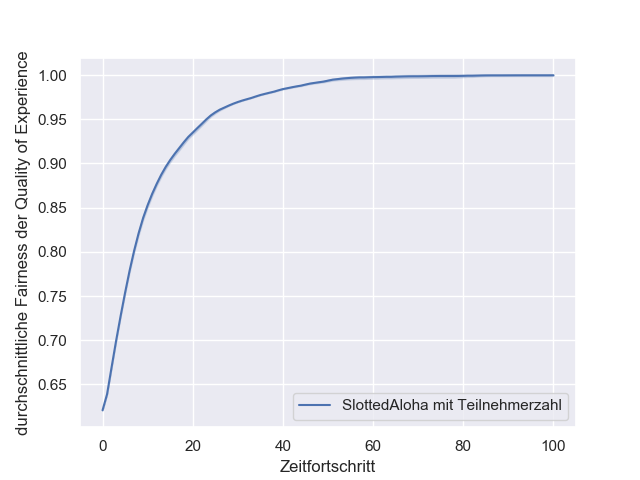
\includegraphics[scale=0.4]{img/SA_par/SlottedAloha_participants_VDE_tau_10_qoe.png}
	\caption{Durchschnittlicher Qualitätserfahrung eines Elektrofahrzeuges}
	\label{Abb_SAparFairness}
\end{figure}
Abbildung \ref{Abb_SAparFairness} zeigt die Fairness der jeweiligen Qualitätserfahrung über den Zeitverlauf der Ladeservices. Die Qualität des Ladeservices hängt ab von der Standardabweichung des Ladezustandes ab. Der schnelle Anstieg des Graphen, in den ersten 20\% der Zeit er höht sich der Wert von etwa 0,65 um etwa 0,3 auf ca. 0,95 und liegt so nach nur 20\% schon nahe am Idealwert von 1. Der Idealwert wird nach etwa 50\% der Zeit erreicht, ab diesem Zeitpunkt herrscht höchstmögliche Fairness zwischen den Teilnehmern.

\subsection{Slotted Aloha mit Teilnehmerzahl und Fahrzeugparametern}
Die Verwendung des Spannungskontrolles, welcher mit Slotted Aloha erweitert wurde und die Teilnehmeranzahl und die Fahrzeugparameter miteinbezieht. Diese Variante des Controller bestimmt mögliche Wartezeiten unter anderem mit der Hilfe von Zufallszahlen. Die Simulation wurde mit 10 verschieden Startwerten für die Bestimmung dieser Zufallszahlen durchgeführt. Dargestellt werde die Ergebnisse eines einzelnen Werktages, allerdings nicht die Ergebnisse eines einzelnen Durchlaufes, sondern der Mittelwert aller Durchläufe samt der zugehörigen Standartabweichung. Es wird der selbe Werktag wie bereits in Kapitel .. verwendet, um die Vergleichbarkeit der Ergebnisse zu gewährleisten. Dargestellt wird die Transformatorlast, die minimalen Werte der Spannung sowie die Anzahl der Teilnehmer, welche Leistung aus dem Netz beziehen. 
\begin{figure}[htb]
\centering
	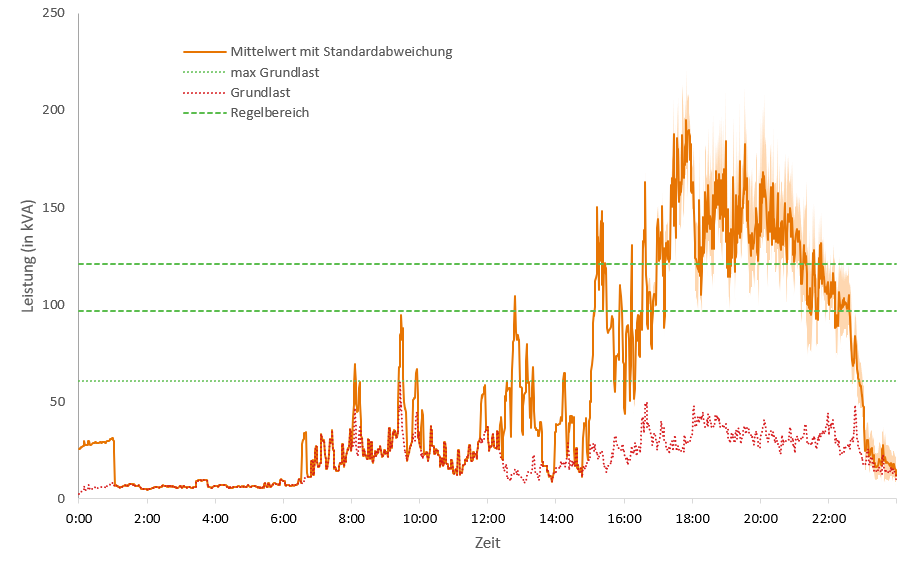
\includegraphics[scale=0.7]{img/SA_wT/TrafoLast3.png}
	\caption{Trafolast bei Verwendung des Spannungs-Controllers ...}
	\label{Abb_SAwtTrafoLast}
\end{figure}

In der Abbildung \ref{Abb_SAwtTrafoLast} ist die vom Transformator ans Niederspannungsnetz abgegeben Scheinleistung in kVA über den Verlauf eines Tages abgebildet. Der Regelbereich des Controllers ist im Falle der Transformatorlast nicht relevant, der VDE Controller lediglich die Spannung berücksichtigt.
\begin{figure}[htb]
\centering
	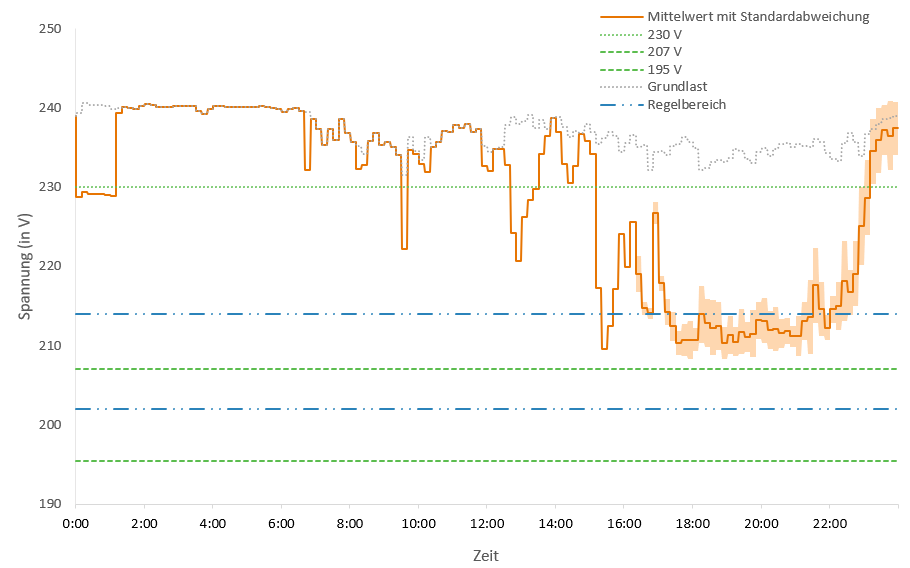
\includegraphics[scale=0.7]{img/SA_wt/Spannung_10m5.png}
	\caption{Spannung bei Verwendung des Spannungs-Controllers ...}
	\label{Abb_SAwtSpannung}
\end{figure}

Abbildung \ref{Abb_SAwtSpannung} zeigt den Verlauf der minimalen Spannung über das gesamte Niederspannungsnetz hinweg. Auch hier werden die Mittelwerte von 10 Minuten Intervallen zur Überprüfung der Norm DIN EN 50160 abgebildet.
\begin{figure}[htb]
\centering
	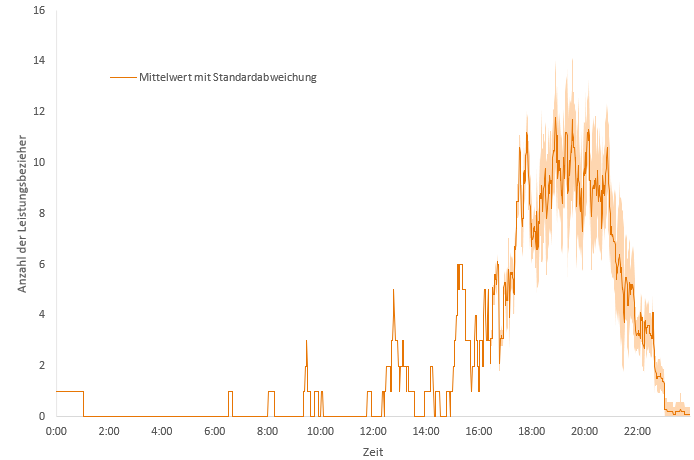
\includegraphics[scale=0.7]{img/SA_wT/Teilnehmer.png}
	\caption{Teilnehmerzahl bei Verwendung des Spannungs-Controllers ...}
	\label{Abb_SAwtTeilnehmer}
\end{figure}

In der Abbildung \ref{Abb_SAwtTeilnehmer} ist die Anzahl an Controllern abgebildet, welche Leistung für das Laden von Elektrofahrzeugen aus dem Netz beziehen. Leistungsbezieher, welche zwar Leistung beziehen, mit dieser aber kein Elektrofahrzeug laden, werden nicht dargestellt. \\
Die Aktivitäten bis etwa 16:00 führen zwar immer wieder zu einem Absinken der Spannung, jedoch erreichen die Werte dabei den Regelbereich des Controllers nicht. Um etwa 16:00 fällt der Spannungswert das erste Mal bis in den Regelbereich hinein ab, erholt sich dann aber wieder. Dieser kurze Abfall lässt sich auf eine kurzfristig ansteigende Anzahl an Teilnehmer und so auch steigende Transformatorlast zurückführen. Von etwa 17:00 bis 21:00 befinden sich die Mittelwerte der Minimalspannung durchgängig im Regelungsbereich des Controllers. Die Werte bewegen sich im Bereich von 217 V bis 210 V, schwanken in diesem Zeitraum also nur um etwa 7 V. Die geringe Schwankung der Werte sowie fehlende Unterschreitungen des Regelbereiches lässt den Schluss zu das diese variante des Controllers dazu in der Lage ist die Spannung effektiv zu regeln und sie auf einem ausreichenden Niveau zu halten.
Im gesamten betrachteten Zeitraum von einer Woche kommt es zu keiner Unterschreitung der 195 Voltmarke sowie zu lediglich im Durchschnitt etwa 0,4 Unterschreitungen der 207 Volt Marke. Die Norm DIN EN 50160 wird folglich erfüllt, da die betrachteten Grenzwerte innerhalb der erlaubten Bereiche liegen.\\
Über den Simulationszeitraum hinweg wurden im Schnitt 392,6 Situationen (+- 12,2\%) festgestellt, in denen Spannungswerte gemessen wurden, welche eine Spannungskollision verursachen könnten. In 246,9 dieser 392,6 Situationen (+- 9,2\%) trat tatsächlich eine Spannungskollision auf und eine Wartezeit wurde berechnet. Der Simulationszeitraum umfasst 10080 Zeitschritte für 110 Teilnehmer, folglich wurden 1108800 Situationen betrachtet. Die 246,9 Situationen stellen also 0,02\% der insgesamt betrachteten Situationen dar. Die hier verwendete Methodik reagiert nur auf Spannungskollisionen, die Menge von Situationen in denen eine Transformatorkollision auftreten könnte wurde dennoch erfasst. In durchschnittlich 9271,5 (+- 3,3\%) der betrachteten Situationen wurde ein Verstoß gegen den Grenzwert der Transformatorlast festgestellt, was etwa 0,83\% aller Situationen entspricht.\\
\begin{figure}
	\begin{subfigure}{0.49\linewidth}
		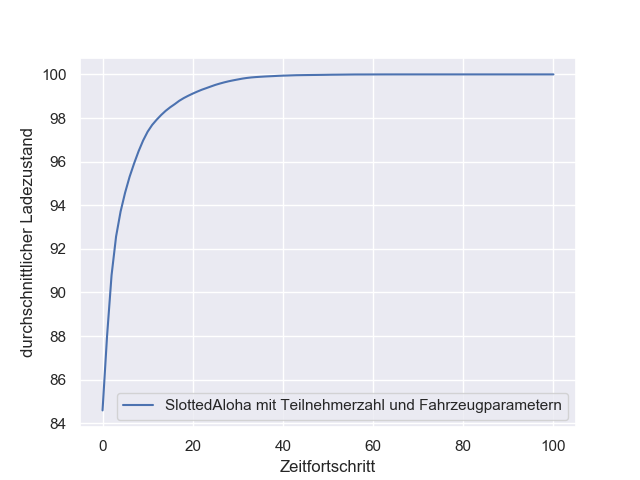
\includegraphics[width=\linewidth]{img/SA_wT/SlottedAloha_waitingTime_VDE_tau_6_soc_mean.png}
        \subcaption{Durchschnittlicher Ladezustand eines Elektrofahrzeuges}
        \label{ABB_SAwtSocMEAN}
	\end{subfigure}
	\begin{subfigure}{0.49\linewidth}
		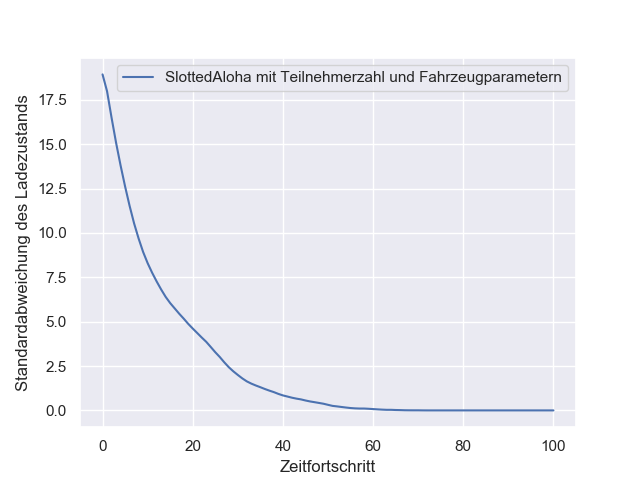
\includegraphics[width=\linewidth]{img/SA_wT/SlottedAloha_waitingTime_VDE_tau_6_soc_std.png}
        \subcaption{Durschschnittliche Standardabweichung des Ladezustandes}
        \label{ABB_SAwtSocSTD}
	\end{subfigure}
	\caption{ganz unten}
\end{figure}

Alle 557 gestarteten Ladeservices wurden erfolgreich abgeschlossen, somit ist die Qualitätserfahrung aller Ladevorgänge maximal. Abbildung \ref{ABB_SAwtSocMEAN} zeigt den durchschnittlichen Ladezustand über den Verlauf eines Ladeservices hinweg, Abbildung \ref{ABB_SAwtSocSTD} zeigt die zugehörige Standardabweichung. Ein schneller Anstieg des mittleren Ladezustands zeigt das Fahrzeuge bereits zu Beginn des jeweiligen Ladeservices mit dem Laden beginnen. Nach etwa 20\% der Zeit hat sich der mittlere Ladestand von etwa 85\% auf etwa 99\% erhöht und hat damit den Zielwert von 100\% fast erreicht. Die zu diesem Zeitpunkt mit etwas unter 5\% ebenfalls bereits gesunkene Standardabweichung weist auf eine Angleichung der jeweiligen Werte hin.\\
\begin{figure}[htb]
\centering
	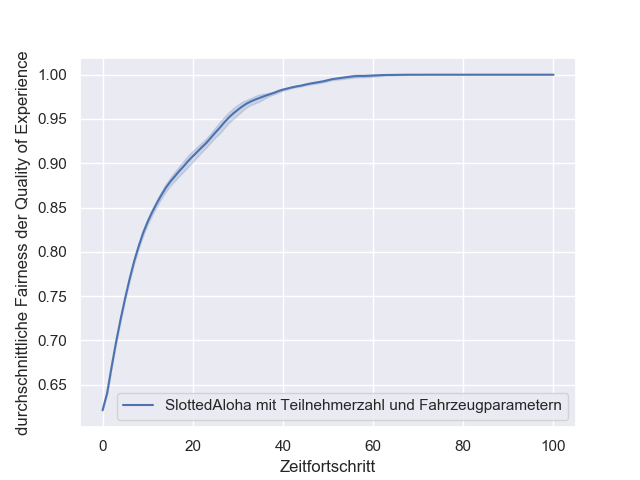
\includegraphics[scale=0.4]{img/SA_wT/SlottedAloha_waitingTime_VDE_tau_6_qoe.png}
	\caption{Durchschnittlicher Qualitätserfahrung eines Elektrofahrzeuges}
	\label{Abb_SAwTFairness}
\end{figure}

Abbildung \ref{Abb_SAwTFairness} zeigt die Fairness der jeweiligen Qualitätserfahrung über den Zeitverlauf der Ladeservices. Die Qualität des Ladeservices hängt ab von der Standardabweichung des Ladezustandes ab. Der schnelle Anstieg des Graphen, in den ersten 20\% der Zeit er höht sich der Wert von etwa 0,65 um etwa 0,25 auf ca. 0,9 und liegt so nach nur 20\% schon nahe am Idealwert von 1. Der Idealwert wird nach etwa 50\% der Zeit erreicht, ab diesem Zeitpunkt herrscht höchstmögliche Fairness zwischen den Teilnehmern.

\subsection{SA-Part-trafo alleine}
\subsection{SA-waitingTime-trafo alleine}
\section{Analyse und Auswertung}
\subsection{SA-part mit SA-waitingTime}
\subsection{SA-part-trafo mit SA-waitingTime-trafo}
\subsection{VDE mit (SA-part, SA-waitingTime)}
\begin{figure}[htb]
\centering
	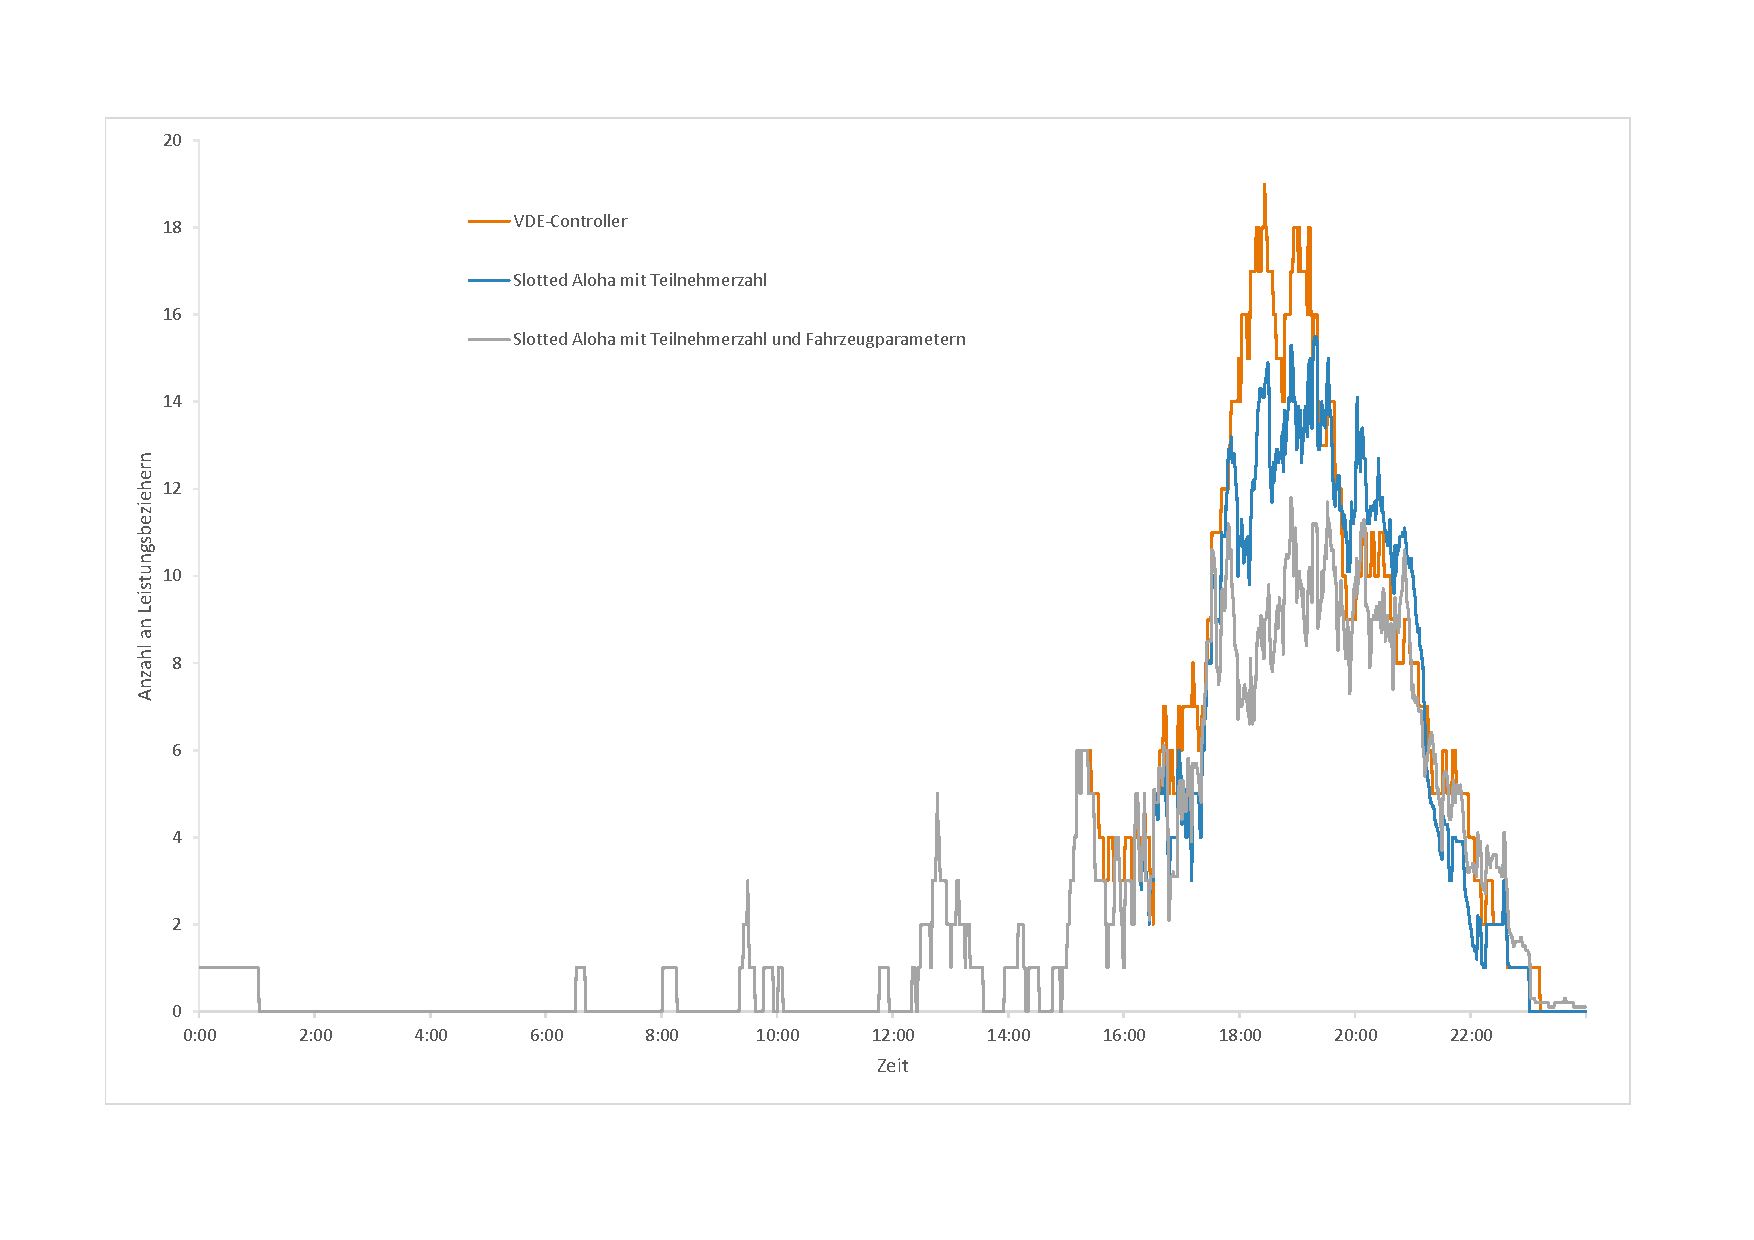
\includegraphics[scale=0.7]{img/ohneTrafo/Teilnehmer2.png}
	\caption{Teilnehmerzahl ohne Trafo}
	\label{Abb_oTTeilnehmer}
\end{figure}

\begin{figure}[htb]
\centering
	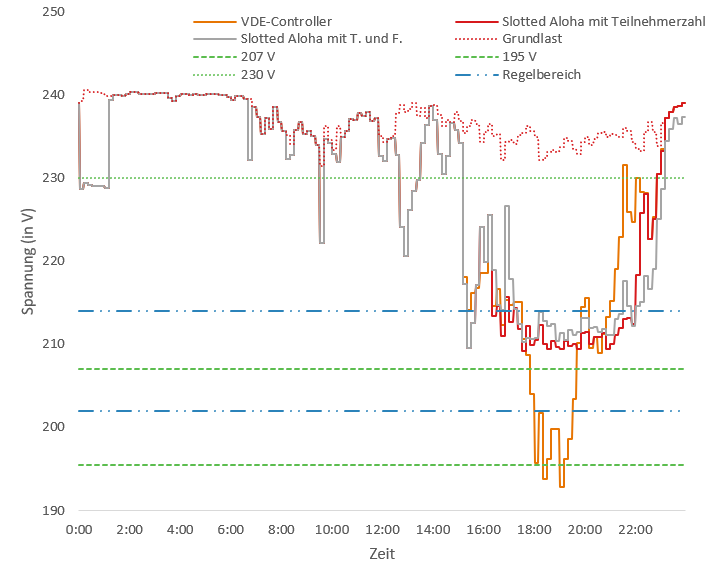
\includegraphics[scale=0.7]{img/ohneTrafo/Spannung2.png}
	\caption{Spannung ohne Trafo}
	\label{Abb_oTSpannung}
\end{figure}

\begin{figure}[htb]
\centering
	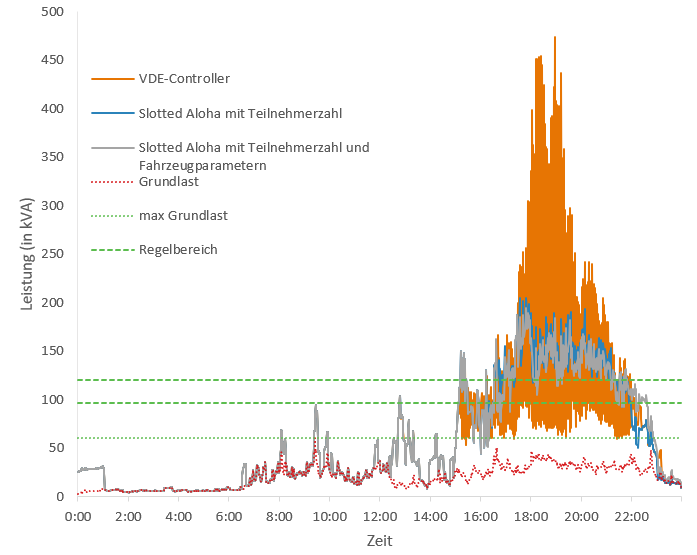
\includegraphics[scale=0.7]{img/ohneTrafo/TrafoLast3.png}
	\caption{Trafolast ohne Trafo}
	\label{Abb_oTTrafo}
\end{figure}

\subsection{(SA-part, SA-waitingTime) mit (SA-part-trafo, SA-waitingTime-trafo)}
